\documentclass{article}
\usepackage{graphics}
\usepackage{hyperref}
\usepackage{natbib}

\begin{document}
\title{Introduction to Information Retrieval}
\author{STA 325, Fall 2018}
\date{October 5, 2018}
\maketitle

\begin{quotation}
  \textsc{Readings:} {\em Principles of Data Mining \url{https://www.amazon.com/Principles-Adaptive-Computation-Machine-Learning/dp/026208290X}}, ch. 1, and sections 14.1
  and 14.3.0--14.3.1.
\end{quotation}


One of the fundamental problems with having a lot of data is finding what
you're looking for.  This is called {\bf information retrieval}.

The oldest approach is to have people create data about the data, {\bf
  metadata}, to make it easier to find relevant items.  Library catalogues are
like this (Figure \ref{fig:metadata}): people devise detailed category schemes
for books, magazines, etc.  For instance, a book has a title, one or more
authors (possibly ``anonymous'' or pseudonyms), a publisher, a place of
publication, a date of publication, possibly an ISBN, and its contents belong
to one or more subject topics, with a lot of work going in to designing the set
of subject-matter topics.  A magazine doesn't have an author, it has multiple
volumes with multiple dates, and it has an ISSN instead of an ISBN, if it has a
number like that at all.  (Nowadays we'd call this sort of scheme an {\bf
  ontology}.)  Having fixed on a scheme like this, people would actually
examine the objects, decide which categories they belong to, and write down
that information along with their location on the shelves, and then copy this
information so that it appeared in multiple places --- by title, by author, by
subject, etc.  This worked OK for a few thousand years, but it needs people,
who are slow and expensive and don't scale.  It's not feasible for searching
census records, or purchase histories at an online store, or the Web.

\begin{figure}
  \resizebox{\textwidth}{!}{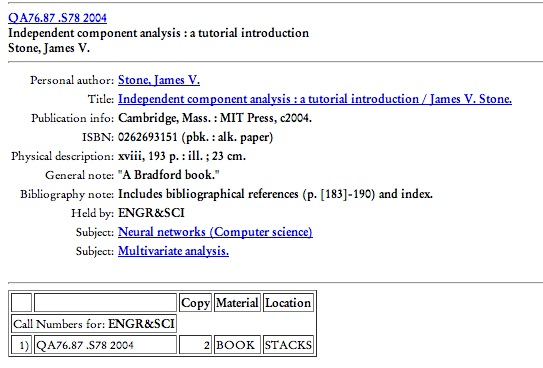
\includegraphics{metadata}}
  \caption{Example of {\bf metadata} (from \texttt{cameo.library.cmu.edu}).
    This is information {\em about} the book, which is not part of its actual
    contents.  Notice that this is {\bf structured}: every book in the
    catalogue will have a title, an author (possibly ``anonymous''), one or
    more subjects, a location, etc.  All of this information is
    humanly-generated.}
  \label{fig:metadata}
\end{figure}


The next oldest approach is Boolean queries: things like ``all census records
of Presbyterian or Methodist plumbers in Rhode Island with at least two but no
more than five children''.  The first electronic data-processing machines were
invented about 120 years ago to do searches like this.  The advantages are that
it's very easy to program, it doesn't need a lot of human intervention, and
sometimes it's exactly what you want to do, say if you're taking a census.  But
there are disadvantages: most people don't think in Boolean queries; it works
best when it's dealing with {\bf structured} data, like census records, not
{\bf unstructured} data like most documents on the Web; and it's got no sense
of {\em priority}.  Suppose you're loking for a used car, thinking of buying a
2001-model-year Saturn, and want to know what problems they're prone to.
Imagine doing a Boolean search of the whole Web for ``Saturn AND 2001 AND
problems''.  {\em Some} of those documents will be just what you want, but
you'll also get a lot about the planet Saturn, about the novel {\em 2001: A
  Space Odyssey} (set at Saturn), and so on.

This is where {\bf searching by similarity} comes in.  Suppose you can find
{\em one} Web page which is about problems in 2001-model Saturns.  We're going
to see today how you can tell your computer ``find me more pages like this''.
We will see later how you can avoid the step of initially lucking into the
first page, and how you can use the same sort of trick to search other kinds of
data --- say images on the Web, or hospital patient records, or retail
transactions, or telephone-call records.

To illustrate these ideas concretely, later in one of our lectures, we're going to use a part of the {\em New
  York Times Annotated Corpus}.  This consists
of $1.8 \times {10}^6$ stories from the {\em Times}, from 1987 to 2007, which
have been hand-annotated with metadata about their contents.  (See Figure
\ref{fig:nytannotated}.)  We are going to look at methods for information
retrieval which do {\em not} use the metadata, but having it there will help us
determine how well those methods are working.  You will get to use a small part
of this data set in class and in one of your homework exercises. (The metadata and annotations are in
  a language called XML.  You will {\em not} have to learn it.)

\begin{figure}
  \resizebox{\textwidth}{!}{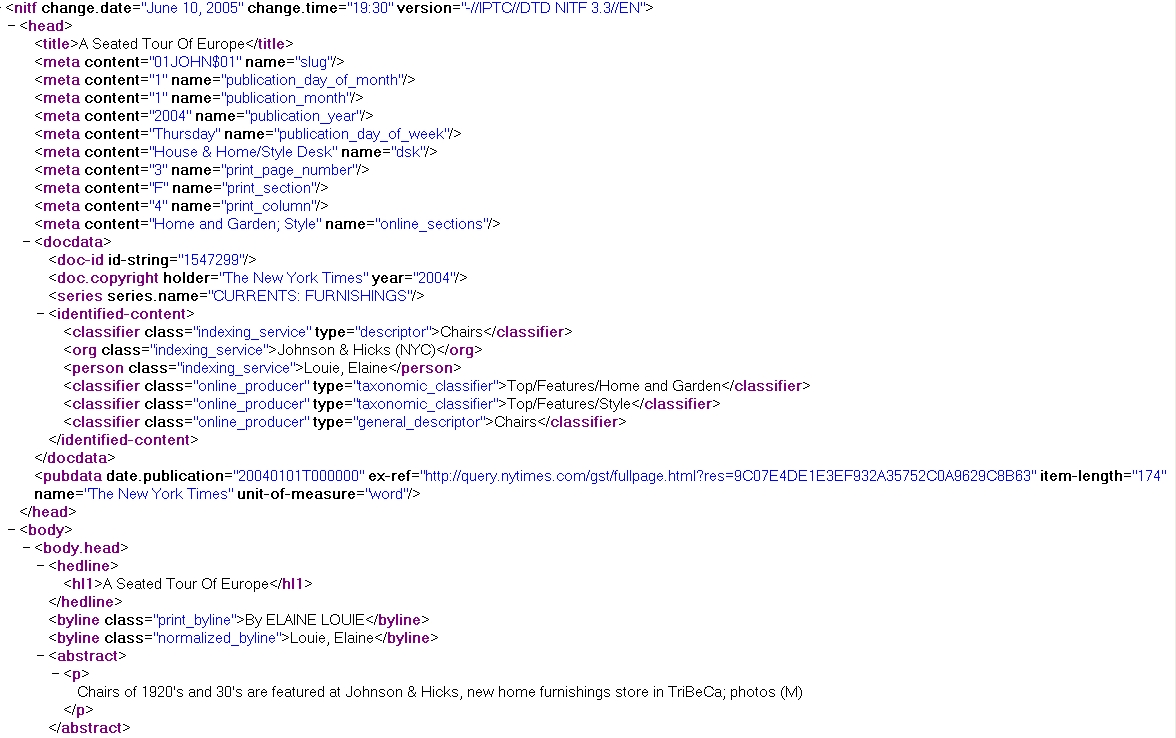
\includegraphics{nytannotated}}
  \caption{Example of the structured meta-data provided with the {\em New York
      Times Annotated Corpus}.  Notice in particular the subject
    classifications.  From
    \url{http://www.ldc.upenn.edu/Catalog/CatalogEntry.jsp?catalogId=LDC2008T19}.
    (Text and annotations copyright by the New York Times Co., used here for
    educational purposes per the terms of the licensing agreement.)}
  \label{fig:nytannotated}
\end{figure}


\section{Representation}

The crucial first step is to chose a representation of the data.  There are
multiple considerations here.
\begin{itemize}
\item The representation ought to be something our methods can work with easily.
\item The representation ought to be something we can easily generate from the
  raw data.
\item The representation ought to highlight the important, helpful aspects of
  the data, and suppress others.  (If the representation {\em didn't} ignore
  some aspects of the data, it would be the data again.)
\end{itemize}
One of the things we'll see is that getting a good representation --- trading
these concerns off against each other --- is at least as important as picking
the right algorithms.

For today, we are searching for documents by similarity, so our data are
natural-language documents.

We could try to represent the {\em meaning} of the documents.  Look Figure
\ref{fig:nytannotated} again.  The abstract reads ``Chairs of the 1920s and 30s
are featured at Johnson \& Hicks, new home furnishing store in TriBeCa''.
We could try to represent the meaning here in something like logical
notation:
\begin{verbatim}
exhibit.of(chairs(age-1920--1930),Johnson&Hicks,now)
is.a(Johnson&Hicks,store,type="home furnishing")
location.of(Johnson&Hicks,TriBeCa)
begin.date(Johnson&Hicks,now)
\end{verbatim}
and then we'd probably want to go on to tell the system that chairs are a kind
of furniture, where TriBeCa is, that chairs that old are a kind of vintage
product, etc.  If we could do this, there are tons of methods for automated
logical reasoning which we could use to find stories about displays of
contemporary chairs, or vintage lamps, etc.  The snag is that extracting this
sort of meaning {\em from the text alone}, without using human readers, turns
out to be insanely hard.  People in artificial intelligence have been saying
it'll happen within the next twenty years for more than fifty years; so we'll
wish them good luck and leave them to their work.

A less ambitious sort of representation which still tries to get more or less
explicitly at meanings would be to draw up a big list of categories, and then
go over the documents and check of which categories they fall in to.  This is
basically what the annotating meta-data does for the {\em Times} corpus.
Social scientists sometimes do this and call it {\bf coding} the documents;
they'll often code for the emotional tone or {\bf valence} as well.  (This
tends to be done with smaller, more focused sets of documents, so they can get
away with smaller sets of categories.)  Once we have this, our representation
is a bunch of discrete variables, and there are lots of methods for analyzing
discrete variables.  But, again, extracting this sort of information {\em
  automatically} from the text is too hard for this to be useful to
us.\footnote{However, we will see later that it is sometimes possible to trick
  people into doing this coding work for us for free.}  In fact, the best
automatic methods for this sort of thing use the bag-of-words representation
which is coming up next.

\subsection{Textual features}

We don't know enough about how people extract meanings from texts to be able to
automate it, but we do know that we extract meanings from texts --- and
different meanings from different texts.\footnote{Conversely, different people
  extract different meanings from the {\em same} texts, raising another set of
  issues, which I will ignore.} This suggests that we should be able to use
{\bf features} or aspects of the text as proxies or imperfect signs of the
actual meanings.  And the text is right there in the computer already, so this
should be easy.  We just have to decide which textual features to use.

Think of what goes on in trying to distinguish between Saturn the brand of car,
Saturn the planet, Saturn the mythological figure, Saturn the type of rocket,
etc.  Documents about all of these will of course contain the word ``Saturn'',
so looking for that word wouldn't help us tell them apart.  However, the {\em
  other} words in the document will tend to differ.  ``Saturn'' together with
words like ``automobile'', ``wheels'', ``engine'', ``sedan'' tends to indicate
the car, whereas words like ``rings'', ``hydrogen'', ``orbit'', ``Titan'',
``Voyager'', ``telescope'', ``Cassini'', etc., indicate the planet.  This
suggests a {\em very} simple representation of the document: all the different
words it contains.

That representation is actually a little {\em too} simple to work well in
practice.  The classic {\bf bag-of-words} (BoW) representation is to list all
of the distinct words in the document together with how often each one appears.
The name comes from imagining printing out the text, cutting the paper into
little pieces so each word is on its own piece, and then throwing all the
pieces into a bag.  This is a definitely set of purely textual features (one
per distinct word), and it's not hard for us to calculate it automatically from
the data.  What remains to be seen is whether we can actually do useful work
with this representation.

\paragraph{Vectors} There are actually two different ways you could
try to code up the bag-of-words, at least as I've described it so far.  
To illustrate this, let's look at the full text of the story featured in Figure \ref{fig:nytannotated} and see how to turn it into a bag of words.
\begin{quotation}
  Lisa Weimer, right, opened her home furnishings store, Johnson \& Hicks, in
  TriBeCa in September, and discovered her passion for chairs, especially those
  from the 1920's and 30's. ''I love simple, clean lines and the richness of
  woods,'' said Ms. Weimer, who was once a home furnishings buyer at Bergdorf
  Goodman.

  A pair of French 1930's walnut chairs with checkerboard backs, above, are
  \$8,500; steel folding chairs from the 1930's, originally used on a French
  ferry, are \$575 each; tubular steel dining chairs upholstered in Ultrasuede,
  right, are 12 for \$14,000. There are 500 chairs, and 100 tables. Johnson \&
  Hicks is at 100 Hudson Street at Franklin Street. Information: (212)
  966-4242.
\end{quotation}

Throwing away punctuation, and treating all numbers as just ``X'', we
get the word-counts in Table \ref{table:wordcounts}

\begin{table}
\begin{verbatim}
           X        1920s        1930s            a        above 
           9            1            3            3            1 
         and          are           at        backs     bergdorf 
           4            3            3            1            1 
       buyer       chairs checkerboard        clean   discovered 
           1            4            1            1            1 
  especially        ferry      folding          for     franklin 
           1            1            1            2            1 
      french         from  furnishings      goodman          her 
           2            2            2            1            2 
       hicks         home       hudson            i           in 
           2            2            1            1            2 
 information           is      johnson        lines         lisa 
           1            1            2            1            1 
        love           ms           of           on         once 
           1            1            2            1            1 
      opened   originally         pair      passion     richness 
           1            1            1            1            1 
       right         said    september       simple        steel 
           2            1            1            1            1 
       store       street       tables          the        there 
           1            2            1            3            1 
       those      tribeca         used       walnut          was 
           1            1            1            1            1 
      weimer          who         with        woods 
           2            1            1            1 
\end{verbatim}
  \caption{Counts of the distinct words in the story, mapping all numbers to ``X''.}
\label{table:wordcounts}
\end{table}

There are (at least) two different data structures we could use to store this
information.  One is a list of {\bf key-value pairs}, also known as an {\bf
  associative array}, a {\bf dictionary} or a {\bf hash}.  The keys here would
be the words, and the associated values would be the number of occurrences, or
count, for each word.  If a word does not appear in a document, that word is
not one of its keys.  Every document would have, in principle, its own set of
keys.  The order of the keys is entirely arbitrary; I printed them out
alphabetically above, but it really doesn't matter.

It turns out, however, that it is a lot more useful to implement bags of words
as {\bf vectors}.  Each component of the vector corresponds to a different word
in the total {\bf lexicon} of our document collection, in a fixed, standardized
order.  The value of the component would be the number of times the word
appears, possibly including zero.

We use this vector bag-of-words representation of documents for two big
reasons:
\begin{itemize}
\item There is a huge pre-existing technology for vectors: people have worked
  out, in excruciating detail, how to compare them, compose them, simplify
  them, etc.  Why not exploit that, rather than coming up with stuff from
  scratch?  (How would you measure the distance between two associate arrays?)
\item In practice, it's proved to work pretty well.
\end{itemize}



% Function to read in a story:
% require(XML)
% fulltext.from.xml <- function(file) {
%   doc <- xmlRoot(xmlTreeParse(file))
%   node.set <- getNodeSet(doc,path="//block[@class='full_text']")
%   text <- sapply(node.set,xmlValue)
%   return(text)
% }
% source("01.R")
% #strip.text() will turn into a text vector
% #table turns into a table
% music.1 <- table(strip.text(fulltext.from.xml("music/0023931.xml")))
% music.2 <- table(strip.text(fulltext.from.xml("music/0345664.xml")))
% music.3 <- table(strip.text(fulltext.from.xml("music/0528767.xml")))
% music.4 <- table(strip.text(fulltext.from.xml("music/0752044.xml")))
% music.5 <- table(strip.text(fulltext.from.xml("music/1658236.xml")))
% art.1 <- table(strip.text(fulltext.from.xml("art/0911479.xml")))
% art.2 <- table(strip.text(fulltext.from.xml("art/1272852.xml")))
% art.3 <- table(strip.text(fulltext.from.xml("art/1346817.xml")))
% art.4 <- table(strip.text(fulltext.from.xml("art/1732382.xml")))
% art.5 <- table(strip.text(fulltext.from.xml("art/1803157.xml")))
% small.bow <- make.BoW.frame(list(music.1,music.2,music.3,music.4,music.5,art.1,art.2,art.3,art.4,art.5),row.names=c("music.1","music.2","music.3","music.4","music.5","art.1","art.2","art.3","art.4","art.5"))
% small.bow[,c("a","against","but","camera","gallery","hit","husband","images","imagined","instruments","melody","new","old","photographs","photography","songs","wife")]

To illustrate, I have taken ten random documents from the {\em Times} corpus
--- five of them about music, five about the arts (excluding music) --- and
turned them all into bag-of-words vectors.\footnote{You will get these
  documents, and more, in the first problem set.}  There were 700 distinct
words in these ten documents (excluding ``singletons'' which only appeared in a
single text).  This means that each document is represented by a vector with
700 components --- that we have 700 features.  Obviously I can't show you these
vectors, but I will show a few of these components (Table
\ref{table:bow-matrix}).

\begin{table}
\begin{verbatim}
         a against but camera gallery hit husband images imagined
music.1 13       0   3      0       0   0       0      0        0
music.2 18       0   7      0       0   2       0      0        0
music.3 33       0   2      0       3   1       0      0        0
music.4 28       0  11      0       0   1       0      0        0
music.5 10       0   0      0       1   0       0      0        0
art.1   20       0   3      2       0   0       1      0        0
art.2   51       0   9      1       4   0       0      2        1
art.3   55       1   6     11       1   0       2      8        0
art.4   64       2   7      0       0   0       0      0        2
art.5   11       1   1      0       0   0       0      2        0

        instruments melody new old photographs photography songs wife
music.1           3      1   0   0           0           0     0    0
music.2           0      0   1   1           0           0     0    0
music.3           0      0   2   1           0           0     3    0
music.4           0      0   2   0           0           0     0    1
music.5           0      1   2   1           0           0     1    0
art.1             0      0   1   0           0           1     0    1
art.2             0      0   3   3           1           4     0    1
art.3             1      0   5   2           0           3     0    2
art.4             0      0   1   0           0           0     0    2
art.5             0      0   0   0           1           1     0    0
\end{verbatim}
  \caption{Bag-of-words vectors for five randomly selected stories classified as ``music'', and five classified as ``art'' (but not music), from the {\em Times} corpus.  The table shows a selection of the 700 features.}
\label{table:bow-matrix}
\end{table}

Things to notice:
\begin{itemize}
\item The data take the form of a matrix.  Each row corresponds to a distinct
  {\bf case} (or instance {\bf instance}, {\bf unit}, {\bf subject}, \ldots)
  --- here, a document --- and each column to a distinct feature.
  Conventionally, the number of cases is $n$ and the number of features is $p$.
  It is no coincidence that this is the same format as the data matrix
  $\mathbf{X}$ in linear regression.
\item Look for contrasts between the documents about music and those about art.
  Some of them (``camera'', ``hit'', ``melody'') you could probably have
  guessed, if you'd thought about it --- but what's going on with ``husband''
  and ``wife'', or ``imagined''?
\item The word ``a'' seems to appear more in stories about art than in stories
  about music.  Why might this be?  Do we really want to pay attention to it?
\item Does it really make sense to distinguish here between ``photographs'' and
  ``photography''?
\end{itemize}


\section{Measuring Similarity}

Right now, we are interested in saying which documents are similar to each
other because we want to do search by content.  But measuring {\bf similarity}
--- or equivalently measuring {\bf dissimilarity} or {\bf distance} --- is
fundamental to data mining.  Most of what we will do will rely on having a
sensible way of saying how similar to each other different objects are, or how
close they are in some geometric setting.  Getting the right measure of
closeness will have a huge impact on our results.

This is where representing the data as vectors comes in so handy.  We already
know a nice way of saying how far apart two vectors are, the ordinary or {\bf
  Euclidean distance}, which we can calculate with the Pythagorean formula:
\[
\| \vec{x} - \vec{y} \| \equiv \sqrt{\sum_{i=1}^{p}{{\left(x_i - y_i\right)}^2}}
\]
where $x_i$, $y_i$ are the $i^{\mathrm{th}}$ components of $\vec{x}$ and
$\vec{y}$.  Remember that for bag-of-words vectors, each distinct word --- each
entry in the lexicon --- is a component or feature.

(The {\bf Euclidean length} or {\bf Euclidean norm} of any vector is
\[
\| \vec{x} \| \equiv \sqrt{\sum_{i=1}^{p}{{x_i^2}}}
\]
so the distance between two vectors is the norm of their difference $\vec{x} -
\vec{y}$.  Equivalently, the norm of a vector is the distance from it to the
origin, $\vec{0}$.)

Now, there are other ways of measuring distance between vectors.  Another
possibility is the {\bf taxicab} or {\bf Manhattan} distance
\[
\sum_{i=1}^{p}{|x_i - y_i|}
\]
It's a perfectly good distance metric; it just doesn't happen to work so well
for our applications.

\subsection{Normalization}

Just looking at the Euclidean distances between document vectors doesn't work,
at least if the documents are at all different in size.
Instead, we need to {\bf normalize} by document size, so that we can fairly
compare short texts with long ones.  There are (at least) two ways of doing
this.

\paragraph*{Document length normalization} Divide the word counts by the total
number of words in the document.  In symbols,
\[
\vec{x} \mapsto \frac{\vec{x}}{\sum_{i=1}^{p}{x_i}}
\]
Notice that all the entries in the normalized vector are non-negative
fractions, which sum to 1.  The $i^{\mathrm{th}}$ component is thus the
probability that if we pick a word out of the bag at random, it's the
$i^{\mathrm{th}}$ entry in the lexicon.

\paragraph*{Euclidean length normalization} Divide the word counts by the
Euclidean length of the document vector:
\[
\vec{x} \mapsto \frac{\vec{x}}{\| \vec{x} \|}
\]
For search, normalization by Euclidean length tends to work a bit better than
normalization by word-count, apparently because the former de-emphasizes words
which are rare in the document.

\paragraph*{Cosine ``distance''} is actually a similarity measure, not a distance:
\[
d_{\cos{}}{\vec{x},\vec{y}} = \frac{\sum_{i}{x_i y_i}}{\| \vec{x}\| \|\vec{y}\|}
\]
It's the cosine of the angle between the vectors $\vec{x}$ and $\vec{y}$.

\newpage

\section{Practice the Criterion of Truth}

I've been pretty free with saying that things work or they don't work, without
being at all concrete about what I mean by ``working''.  We are going to see
many, many different ways of elaborating on ``working'', but for right now, a
first cut is to look at how often the most-similar document is in the wrong
class.  (This obviously relies on our having access to pre-assigned
classes.)

% rownames(small.bow)[nearest.points(small.bow)]
% rownames(small.bow)[nearest.points(div.by.sum(small.bow))]
% rownames(small.bow)[nearest.points(div.by.euc.length(small.bow))]
% would've been slicker to cbind these three...

\begin{table}[h]
\begin{tabular}{l|lll}
& \multicolumn{3}{c}{Best match by similarity measure}\\
& Euclidean & Euclidean + word-count & Euclidean + length\\
\hline
music.1 & art.5 & art.4 & art.4\\
music.2 & art.1 & music.4 & music.4\\
music.3 & music.4 & music.4 & art.3\\
music.4 & music.2 & art.1 & art.3\\
music.5 & art.5 & music.3 & music.3\\
art.1 & music.1 & art.4 & art.3\\
art.2 & music.4 & art.4 & art.4\\
art.3 & art.4 & art.4 & art.4\\
art.4 & art.3 & art.3 & art.3\\
art.5 & music.1 & art.3 & art.3\\
\hline
error count & 6 & 2 & 3
\end{tabular}
\caption{Closest matches for the ten documents, as measured by the distances
  between bag-of-words vectors, and the total error count (number of documents
  whose nearest neighbor is in the other class).}
\label{table:matches-and-errors}
\end{table}

This shows that normalization definitely helps, but the difference here between
normalizing by word-count and normalizing by Euclidean length is small, and if
anything in the opposite direction from what I promised.  That promise will,
however, be fulfilled as we go forward, starting next time when we look at how
to do search and classify documents.


\end{document}
